\chapter{Technical Description and Implementation}

\section{System Requirements and Prerequisites}
The implementation of SmartERP utilized standard full-stack development tooling:
\begin{itemize}
    \item \textbf{Development Environment}: Node.js (v18.0+), npm (v9.0+), TypeScript 5.0, Git.
    \item \textbf{Frontend Stack}: Next.js 16.2.9 (App Router, React 19), Tailwind CSS v4, Lucide Icons.
    \item \textbf{Backend Stack}: Node.js, Express.js 4.19, JSON Web Tokens (JWT), bcrypt.js.
    \item \textbf{Data Persistence Layer}: Prisma ORM 6.0, SQLite / PostgreSQL relational database.
    \item \textbf{Document Services}: PDFKit (Vector PDF Invoices), ExcelJS (Spreadsheet Workbooks).
\end{itemize}

\section{System Architecture and Design}
SmartERP follows a decoupled, three-tier microservice-inspired client-server architecture as depicted in Figure~\ref{fig:architecture}.

\begin{figure}[htbp]
  \centering
  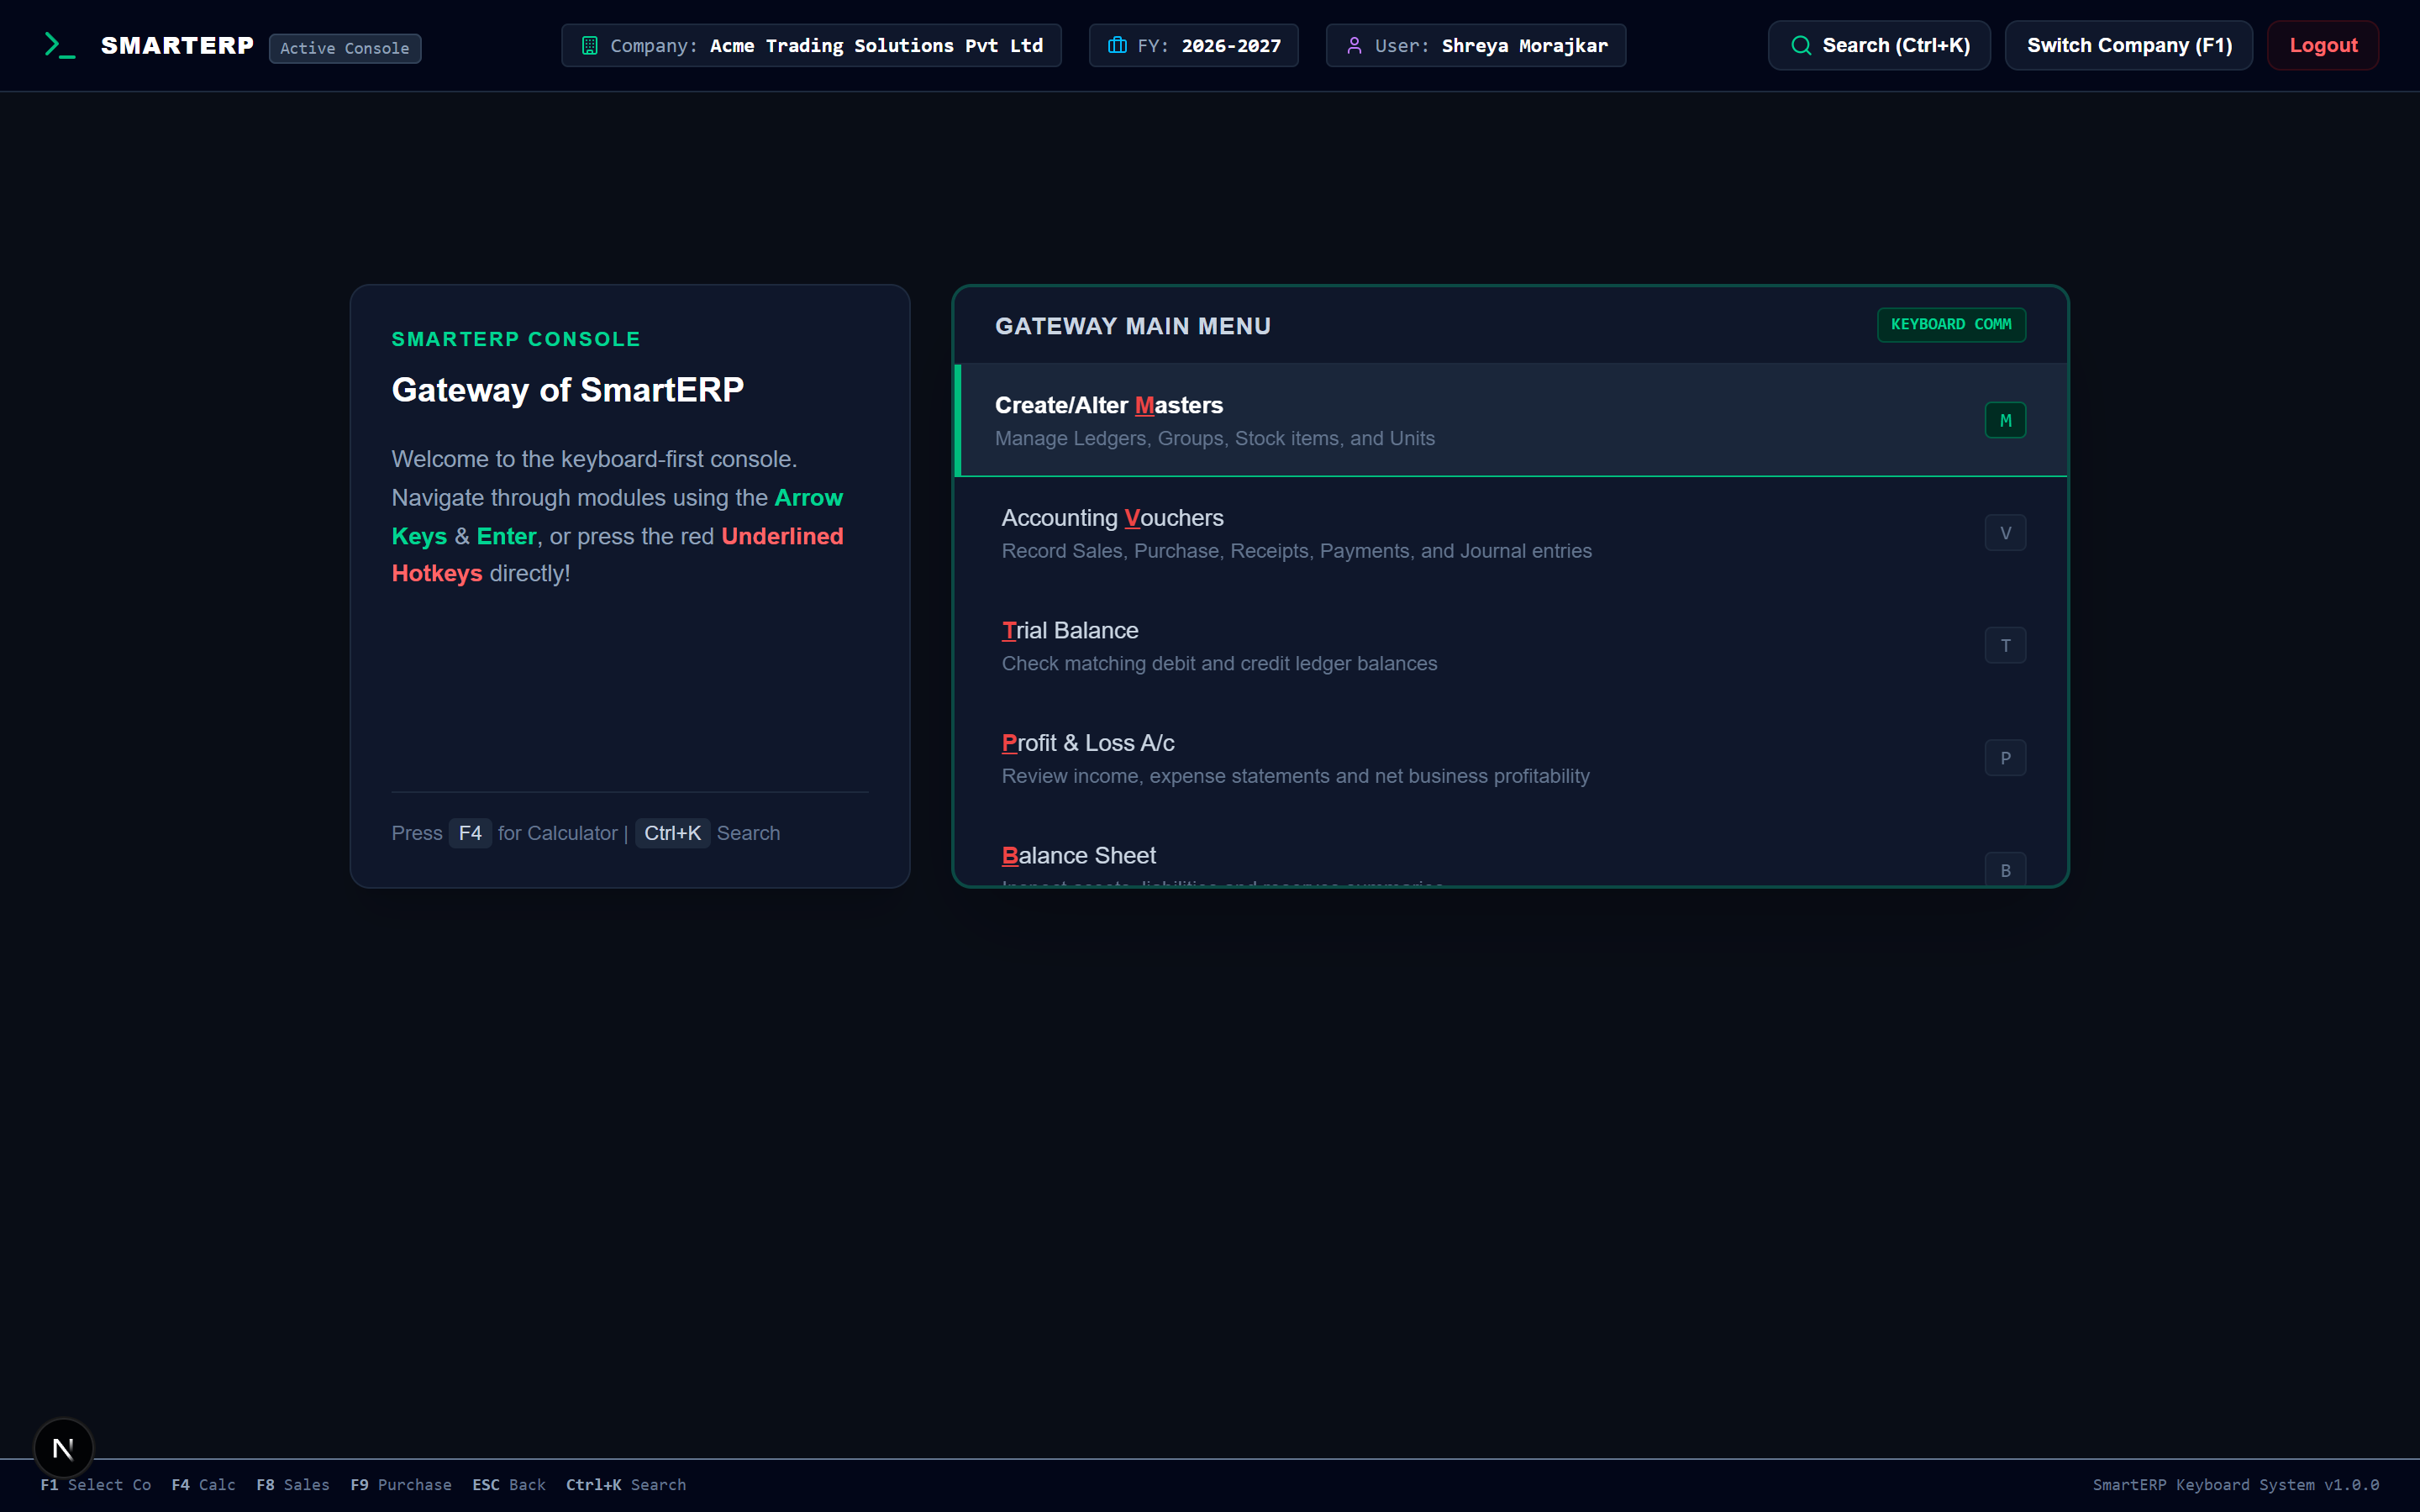
\includegraphics[width=0.85\textwidth]{images/03_gateway_dashboard.png}
  \caption{Gateway Dashboard of SmartERP displaying hotkey-driven navigation}
  \label{fig:architecture}
\end{figure}

The application flow comprises:
\begin{enumerate}
    \item \textbf{Presentation Layer}: Next.js React components rendering reactive ledger grids, voucher allocation tables, and financial statements. Global keyboard events are captured via a dedicated \texttt{useKeyboardShortcuts} React hook.
    \item \textbf{Application \& Business Layer}: Express.js REST API providing modular endpoints for authentication, company management, master creation, voucher processing, tax calculations, and file generation.
    \item \textbf{Database \& ORM Layer}: Prisma ORM mapping type-safe schema definitions into transactional SQL queries, guaranteeing ACID compliance for financial mutations.
\end{enumerate}

\section{Database Modeling and Schema Design}
The relational database schema is structured around double-entry accounting principles and multi-tenant isolation. Table~\ref{tab:schema-summary} summarizes the primary database models.

\begin{table}[htbp]
\centering
\caption{SmartERP Primary Database Entities and Relationships}
\label{tab:schema-summary}
\begin{tabular}{llp{7.5cm}}
\toprule
\textbf{Entity Name} & \textbf{Primary Key} & \textbf{Functional Description} \\
\midrule
\texttt{User} & \texttt{id} (UUID) & System administrator credentials with bcrypt-hashed passwords. \\
\texttt{Company} & \texttt{id} (UUID) & Multi-tenant business workspace with GSTIN and state info. \\
\texttt{Group} & \texttt{id} (UUID) & Chart of Accounts categories (\textit{Assets, Liabilities, Income, Expenses}). \\
\texttt{Ledger} & \texttt{id} (UUID) & Individual party and nominal accounts maintaining current balances. \\
\texttt{StockItem} & \texttt{id} (UUID) & Inventory items with SKU, HSN, rates, GST \%, and stock counts. \\
\texttt{Voucher} & \texttt{id} (UUID) & Transaction header storing type (\textit{SALES, PURCHASE, etc.}) and total. \\
\texttt{VoucherEntry} & \texttt{id} (UUID) & Atomic double-entry lines recording debit and credit amounts. \\
\texttt{GSTRecord} & \texttt{id} (UUID) & Tax audit records recording CGST, SGST, and IGST breakdowns. \\
\bottomrule
\end{tabular}
\end{table}

\section{Core Modules Implementation}

\subsection{Multi-Tenant Company Initialization and Auto-Seeding}
Upon creating a new company, the backend executes an atomic transaction that provisions the company record and seeds the four primary accounting groups along with default system ledgers:
\begin{itemize}
    \item \textbf{Primary Groups}: \textit{Assets (ASSET), Liabilities (LIABILITY), Income (INCOME), Expenses (EXPENSE)}.
    \item \textbf{System Ledgers}: \textit{Cash (Asset), Bank (Asset)}.
\end{itemize}

\subsection{Double-Entry Voucher and Inventory Transaction Engine}
When a user records a voucher (e.g., Sales or Purchase), the backend executes a Prisma transaction (\texttt{tx.\$transaction}) ensuring all balance and stock updates occur atomically:
\begin{enumerate}
    \item Creates the parent \texttt{Voucher} record with unique sequence numbering.
    \item Writes individual \texttt{VoucherEntry} debit and credit records.
    \item Mutates the current balance of affected ledgers:
    \begin{equation}
      \text{Balance}_{\text{new}} = 
      \begin{cases}
        \text{Balance}_{\text{old}} + \text{Debit} - \text{Credit}, & \text{for Asset / Expense Ledgers} \\
        \text{Balance}_{\text{old}} + \text{Credit} - \text{Debit}, & \text{for Liability / Income Ledgers}
      \end{cases}
    \end{equation}
    \item Adjusts inventory quantities (\texttt{currentQty}) in \texttt{StockItem} based on transaction direction ($+\Delta q$ for Purchase, $-\Delta q$ for Sales).
    \item Computes and records applicable GST splits in \texttt{GSTRecord}.
\end{enumerate}

\subsection{State-Aware GST Computation Algorithm}
Algorithm~\ref{alg:gst} formalizes the automated tax determination logic implemented in the billing pipeline.

\begin{algorithm}[htbp]
\caption{State-Aware GST Tax Allocation Engine}
\label{alg:gst}
\begin{algorithmic}[1]
\Require Company State $S_c$, Counterparty State $S_p$, Taxable Amount $A$, GST Rate $R$
\Ensure Total Tax $T$, Tax Breakdown $(\text{CGST}, \text{SGST}, \text{IGST})$
\State $T \gets A \times \left(\frac{R}{100}\right)$
\If{$\text{Normalize}(S_c) = \text{Normalize}(S_p)$} \Comment{Intra-State Transaction}
    \State $\text{CGST} \gets \frac{T}{2}$
    \State $\text{SGST} \gets \frac{T}{2}$
    \State $\text{IGST} \gets 0$
\Else \Comment{Inter-State Transaction}
    \State $\text{CGST} \gets 0$
    \State $\text{SGST} \gets 0$
    \State $\text{IGST} \gets T$
\EndIf
\State \Return $T, (\text{CGST}, \text{SGST}, \text{IGST})$
\end{algorithmic}
\end{algorithm}

\subsection{Keyboard Navigation and Productivity Engine}
To provide high-speed data entry, a custom React hook intercepts browser keyboard events:
\begin{itemize}
    \item \textbf{Function Keys}: $F1$ (Switch Company), $F4$ (Floating Calculator Overlay), $F8$ (Sales Voucher), $F9$ (Purchase Voucher), $F5$--$F7$ (Payment, Receipt, Journal).
    \item \textbf{Spotlight Search ($Ctrl+K$)}: Opens a fuzzy-search palette to jump instantly to any ledger, item, or report.
    \item \textbf{Underlined Hotkeys}: Pressing highlighted hotkey letters directly on menu cards ($M$ for Masters, $V$ for Vouchers, $T$ for Trial Balance) triggers immediate routing.
\end{itemize}

\begin{figure}[htbp]
  \centering
  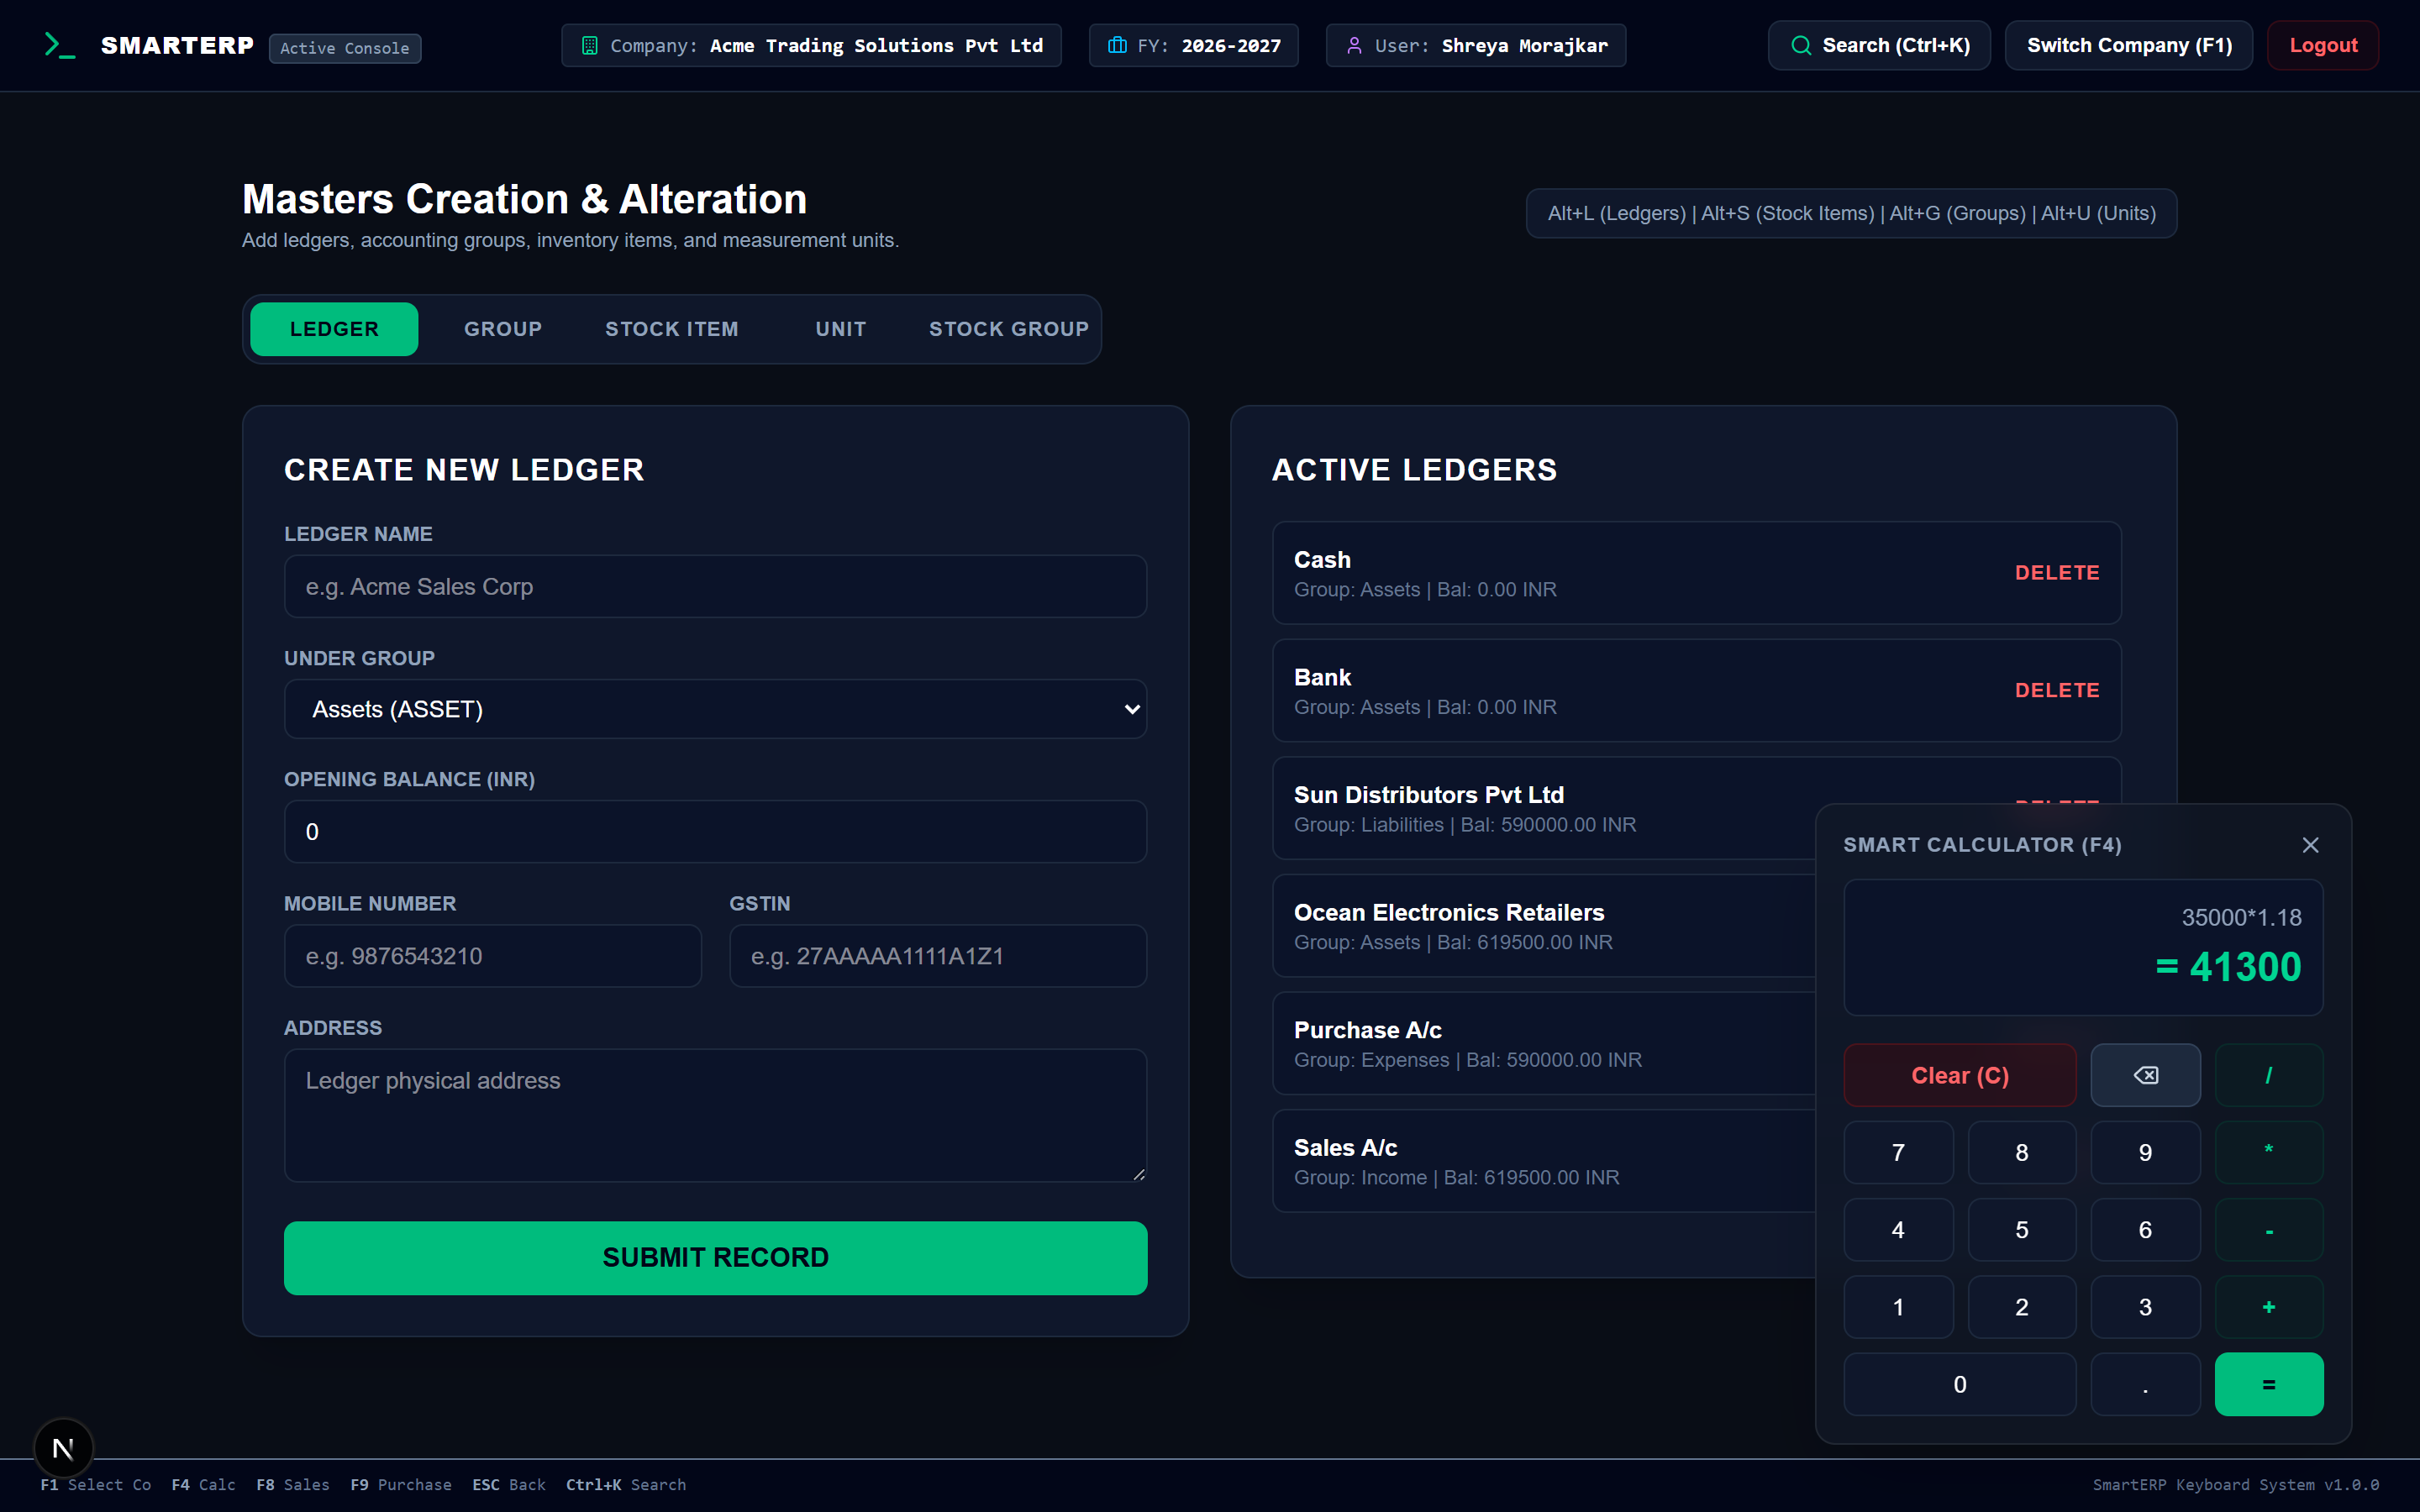
\includegraphics[width=0.85\textwidth]{images/04_calculator_overlay.png}
  \caption{Context-preserving floating calculator overlay ($F4$) during ledger management}
  \label{fig:calculator}
\end{figure}

\subsection{Real-Time Financial Reporting and Verification}
Financial statements are dynamically generated from ledger entries:
\begin{itemize}
    \item \textbf{Trial Balance}: Computes cumulative debits ($\sum Dr$) and credits ($\sum Cr$) verifying the fundamental accounting equation:
    \begin{equation}
      \sum_{i=1}^{n} \text{Debit}_i = \sum_{j=1}^{m} \text{Credit}_j
    \end{equation}
    \item \textbf{Profit \& Loss Account}: Computes Gross and Net Income derived from total Income ledger credits minus Expense ledger debits.
    \item \textbf{Balance Sheet}: Verifies that $\text{Total Assets} = \text{Total Liabilities} + \text{Equity/Reserves}$.
    \item \textbf{Stock Valuation}: Evaluates warehouse asset value:
    \begin{equation}
      \text{Valuation} = \sum_{k=1}^{p} (\text{CurrentQty}_k \times \text{PurchaseRate}_k)
    \end{equation}
\end{itemize}

\section{Automated Integration Testing and Results}
An automated test harness (\texttt{test\_features.js}) was developed to validate all accounting operations programmatically. Table~\ref{tab:test-results} summarizes the validation results.

\begin{table}[htbp]
\centering
\caption{Automated Integration Test Verification Results}
\label{tab:test-results}
\begin{tabular}{lp{6.0cm}cc}
\toprule
\textbf{Test Module} & \textbf{Verification Target} & \textbf{Expected Output} & \textbf{Status} \\
\midrule
User Authentication & Admin registration \& JWT issuance & Token Generated & \textbf{PASS} \\
Company Seeding & Auto-creation of 4 groups \& 2 ledgers & Groups/Ledgers Verified & \textbf{PASS} \\
Purchase Voucher & Inward 20 TVs @ \text{INR} 25k + 18\% GST & Stock: 120, Liab: \text{INR} 590k & \textbf{PASS} \\
Sales Voucher & Outward 15 TVs @ \text{INR} 35k + 18\% GST & Stock: 105, Asset: \text{INR} 619.5k & \textbf{PASS} \\
Trial Balance & Mathematical balance of Debits vs Credits & $\sum Dr = \sum Cr$ & \textbf{PASS} \\
GST Register & Intra-state CGST + SGST tax allocation & CGST: 50\%, SGST: 50\% & \textbf{PASS} \\
PDF Invoice Export & Vector PDF generation with HSN \& GST & HTTP 200 (application/pdf) & \textbf{PASS} \\
Excel Export & Spreadsheet workbook generation & HTTP 200 (.xlsx stream) & \textbf{PASS} \\
\bottomrule
\end{tabular}
\end{table}
